\ifx\allfiles\undefined
\documentclass[12pt]{book}
\usepackage[a4paper]{geometry}
\usepackage[dvipsnames]{xcolor}
\usepackage{amsmath, amsthm, amssymb, mathrsfs}
\usepackage{graphicx}
\usepackage{enumitem}

\usepackage{tikz}
\usepackage[colorlinks,linkcolor=black]{hyperref}
%\usepackage{biblatex}

\pagestyle{plain}

\graphicspath{ {fig/},{../fig/}, {config/}, {../config/} }

\geometry{top=25.4mm,bottom=25.4mm,left=20mm,right=20mm,headheight=2.17cm,headsep=4mm,footskip=12mm}
\linespread{1.5}
\setenumerate[1]{itemsep=5pt,partopsep=0pt,parsep=\parskip,topsep=5pt}
\setitemize[1]{itemsep=5pt,partopsep=0pt,parsep=\parskip,topsep=5pt}
\setdescription{itemsep=5pt,partopsep=0pt,parsep=\parskip,topsep=5pt}

% Theorem environment
\newtheorem{defn}{Definition}[section]

\newtheorem{lemma}{Lemma}[section]
\newtheorem{theorem}[lemma]{Theorem}
\newtheorem{corollary}[lemma]{Corollary}
\newtheorem{criterion}[lemma]{Criterion}

\newtheorem{proposition}{Proposition}[section]
\newtheorem{example}{Example}[section]
\newtheorem*{rmk}{Remark}


\def\d{\textup{d}}
\begin{document}
% \title{{\Huge Lecture-Notes on \\ \textbf{
Computational Methods in Evolutionary Biology}}}
\author{Chang Longxiao\\
longxiao.chang@campus.lmu.de}
\date{\today}

\maketitle                   % title in a newpage

\thispagestyle{empty}        % without page number
\begin{center}
    \Huge\textbf{FOREWORD}
\end{center}

"\textit{Nothing in biology makes sense except in the light of evolution}," said Theodosius Dobzhansky. Likewise, we could say that \textit{nothing in evolution makes sense except in the light of mathematics}.

As a child, I was fascinated by the vivid beauty of nature. As I grew older, this fascination led me to biology—the science that seeks to describe the dynamics of the living world. However, such descriptions often feel too imprecise, if not unscientific, to truly grasp the complexities of reality. Contrary to what many experimental biologists believe, There is too less mathematic languages used in biology, not too much.
%biology does not suffer from an excess of mathematics, but rather from a shortage of it.

Evolution, as the most fundamental and important topic in biology, appears to have the clearest structure that can be described mathematically, largely due to its long time scale. This note serves as a record of the models and methods I have learned in evolutionary biology. By building upon previous research, we may one day uncover a deeper understanding of the intricate complexity of life.

\begin{flushright}
    \begin{tabular}{c}
        \today \\ 
        Im Biozentrum LMU
    \end{tabular}
\end{flushright}

\iffalse
\begin{center}
    If people do not believe that mathematics is simple,

    it is only because they do not realize how complicated life is. 
    
    ——John von Neumann
\end{center}
\fi

\newpage                   
\pagestyle{plain}             
\setcounter{page}{1}          
\pagenumbering{Roman}    

\tableofcontents              

\newpage                   
\pagestyle{plain}
\setcounter{page}{1}          
\pagenumbering{arabic} 
\else
\fi

\chapter{Phylogenetic Reconstruction from a Probabilistic Perspective}

    We have already discussed distance-based phylogenetic trees and parsimony trees. By using these different algorithms, each based on distinct principles, we aim to find the most probable tree (rather than a 'true' tree) from the given dataset. This fact prompts us to consider phylogenetic reconstruction from a probabilistic perspective.

    In probabilistic terms, we are inferring a phylogenetic tree that best explains the observed sequence data. Firstly, let us consider the example of a coin toss: if we roll a coin $1000$ times and count the number of times it shows 'heads', the observed count of 'heads' (data, D) helps us infer the probability of 'heads' (parameter, p), which is intrinsic to the coin. If we observe 501 'heads,' we might reasonably estimate that p is closer to $0.5$ than to $0.1$ or $0.9$. This intuition comes from noting that, if $p = 0.5$, it is more probable to obtain a result close to $501$ 'heads' than if $p = 0.1$ or $p = 0.9$. In other words, we are inferring the parameter by examining the conditional probability of the observed data given different parameter values.

    \begin{figure}[htbp]
        \centering
        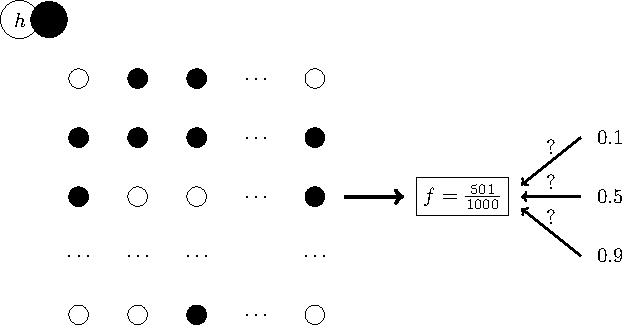
\includegraphics[scale = 0.8]{/coin_toss.pdf}
    \end{figure}

    Returning to phylogenetic reconstruction, our observed data consists of the sequence data ($D$), from which we aim to infer the tree structure ($T$). Calculating the exact probability of a particular tree given the data is challenging, or even impossible. However, similar to inferring the probability of heads in a coin toss, we can calculate the conditional probability of observing the sequence data given a specific tree:
    \begin{equation*}
        Pr(D|T) = ?
    \end{equation*}

    \section{Conditional Probability of Sequence Data Given a Tree}
    
        A basic assumption is that all alignment columns evolve independently of each other. Please note that this assumption does not always hold true. For instance, in the so-called 'CpG' sites — DNA regions where a cytosine is followed by a guanine — the cytosine is more likely to be methylated and subsequently mutate into thymine. In this case, the mutation G $\rightarrow$ T depends on the state of the adjacent site (whether it is a C or not). Despite this, we focus here on the general case where all alignment columns are assumed to be independent. Under this independence assumption, the probability of the data $D$ given the tree $T$ is expressed as:
        \begin{equation}
            Pr(D|T) = \prod_{i} Pr(d_i|T)
        \end{equation}
        
        where $d_i$ represents the $i$th alignment column. 

        \begin{figure}[htbp]
            \centering
            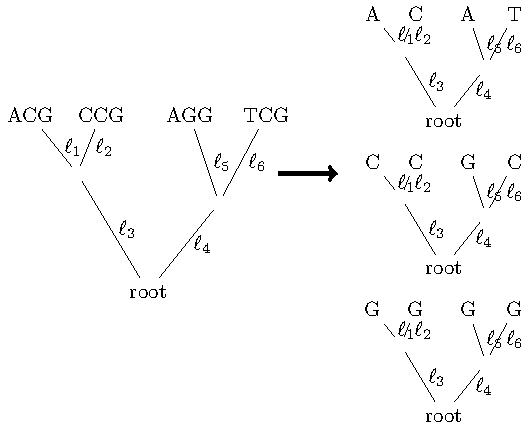
\includegraphics{tree_1_diagram.pdf}
        \end{figure}

        For a tree where the state of each inner node is specified, it is straightforward to calculate the probability of that particular tree.
        
        \begin{figure}[htbp]
            \centering
            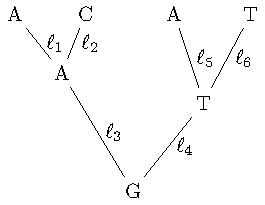
\includegraphics[scale = 1]{tree_1_nucleotide.pdf}
        \end{figure}

        We assume that the probability of a nucleotide $x$ being replaced by $y$ depends on the branch length $\ell$ and is represented by $P_{x \rightarrow y}(\ell)$. Additionally, the probability that the root has state $x$ is denoted as $p_x$. For example, for tree $T_1$ with specified states at the inner nodes, its probability can be calculated as:

        \begin{align*}
            Pr(D|T) &= p_G \cdot P_{G \rightarrow A}(\ell_3) \cdot P_{G \rightarrow T}(\ell_4)
            &\cdot P_{A \rightarrow A}(\ell_1) \cdot P_{A \rightarrow C}(\ell_2)
            &\cdot P_{T \rightarrow A}(\ell_5) \cdot P_{T \rightarrow T}(\ell_6)
        \end{align*}

        However, the states of the inner nodes are usually unknown. As a result, the probability of the tree cannot be directly calculated by simply multiplying all the replacement probabilities along each branch, since the replacements themselves are not determined.
        
        Notice that there are many duplicated calculations when different trees share the same subtree. For Example, consider ((A,T):A,T) and ((A,T):A,G).

        So, what can we do? The simplest approach is to calculate probabilities for every possible combination of inner node states. This involves assigning each inner node one of the four nucleotides $(A, C, G, T)$ and iterating through all possible configurations.

        However, a more effcient approach is to use \textbf{Felsenstein's pruning algorithm}.
    
            \begin{defn}{\textbf{Felsenstein's Pruning Algorithm}}\\
                For each node $k$ let $D_k$ be the part of the data $d_i$ that are labeled to tips that stem from $k$ and define
                    \begin{equation*}
                        w_k(x) = Pr(D_k|\text{$ k $ has an $ x $ at this site})
                    \end{equation*}
                    for every nucleotide $x$.

                    \begin{center}
                        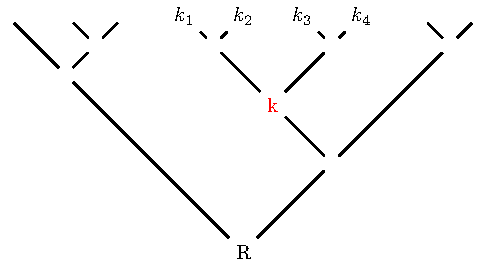
\includegraphics{/Felstein_diagram_k.pdf}
                    \end{center}
                        
                    For any leave $b$ with nucleotide $y$ we have
                        \begin{equation*}
                            w_b(x) = 
                            \begin{cases}
                                0, \text{ if } x \neq y\\
                                1, \text{ if } x = y\\
                            \end{cases}
                        \end{equation*}
            
                    If $k$ is a node with child nodes $i$ and $j$ and corresponding branch lengths $\ell_i$ and $\ell_j$, then
                        \begin{equation}\label{eq:\thesection:F-P_algorithm1}
                            w_k(x) = 
                            \left( \sum_{y \in \{ A, C, G, T\}} P_{x \rightarrow y}(\ell_i) \cdot w_i(y) \right) \cdot
                            \left( \sum_{z \in \{ A, C, G, T\}} P_{x \rightarrow z}(\ell_j) \cdot w_j(z) \right)
                        \end{equation}
                    
                    \begin{center}
                        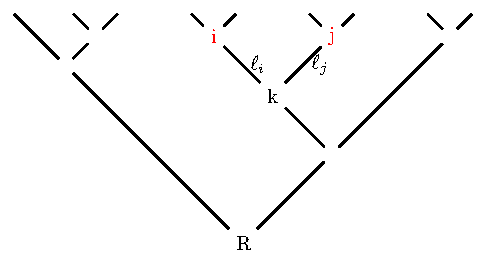
\includegraphics{/Felstein_ij.pdf}
                    \end{center}
            
                    Compute all $w_k(x)$ from the tips to the root by dynamic programming for all $k$ and all $x$. Then for the root $r$ we can compute:
                        \begin{equation}
                            Pr(T|D) = \sum_{x \in \{ A, C, G, T\}} p_x \cdot w_r(x)
                        \end{equation}
                    where $p_x$ is the probability that the root node have the state $x$.
                \end{defn}
        
        A more concise way to express \eqref{eq:\thesection:F-P_algorithm1} is in matrix form. Let $W_k$ represent the matrix of $w_{k,s}(x)$ where $k$ denotes the node, $s$ indicates the sequence position ($n$ positions in total), and $x$ represent the nucleotide:
        \begin{equation*}
            W_k = \left(
                \begin{matrix}
                    w_{k,1}(A) & w_{k,2}(A) & w_{k,3}(A) & \dots & w_{k,n}(A) \\
                    w_{k,1}(C) & w_{k,2}(C) & w_{k,3}(C) & \dots & w_{k,n}(C) \\
                    w_{k,1}(G) & w_{k,2}(G) & w_{k,3}(G) & \dots & w_{k,n}(G) \\
                    w_{k,1}(T) & w_{k,2}(T) & w_{k,3}(T) & \dots & w_{k,n}(T)
                \end{matrix}
            \right)
        \end{equation*}
        
        \textbf{Matrix multiplication}
        $A \cdot B = C$, also called Matmul Product, in which $c_{ij} = \sum_{k=1}^m a_{ik} \cdot b_{kj}$.

        \textbf{Entrywise product}
        $A \circ B = D$, also called Hadamard Product, in which $d_{ij} = a_{ij} \cdot b_{ij}$

        And we define a transition matrix $P(\ell_i) = \left( P_{x \rightarrow y}(\ell_i) \right)_{x,y \in \{ A,C,G,T \}}$ which encapsulates all transition probabilities with the branch length of $\ell_i$:
        \begin{equation*}
            P(\ell_i) = \left(
                \begin{matrix}
                    P_{A \rightarrow A}(\ell_i) & P_{A \rightarrow C}(\ell_i) & P_{A \rightarrow G}(\ell_i) & P_{A \rightarrow T}(\ell_i) \\
                    P_{C \rightarrow A}(\ell_i) & P_{C \rightarrow C}(\ell_i) & P_{C \rightarrow G}(\ell_i) & P_{C \rightarrow T}(\ell_i) \\
                    P_{G \rightarrow A}(\ell_i) & P_{G \rightarrow C}(\ell_i) & P_{G \rightarrow G}(\ell_i) & P_{G \rightarrow T}(\ell_i) \\
                    P_{T \rightarrow A}(\ell_i) & P_{T \rightarrow C}(\ell_i) & P_{T \rightarrow G}(\ell_i) & P_{T \rightarrow T}(\ell_i) \\
                \end{matrix}
            \right)
        \end{equation*}

        Thus, the equation \eqref{eq:\thesection:F-P_algorithm1} can be written as:
        \begin{equation}
            W_k = \left( P(\ell_i) \cdot W_i \right) \circ \left( P(\ell_j) \cdot W_j \right)
        \end{equation}

    \section{Jukes-Cantor Model: Sequence Evolve as a Stochastic Process}

        To calculate the probability of a certain tree using Felsenstein's pruning algorithm, we require both the nucleotide transition probabilities ($P_{x \rightarrow y}$) and the initial distribution of nucleotides ($p_x$). Firstly, consider a discrete time condition: in each generation, the probability of a mutation occurring is $p$. Let $X$ represent a random variable indicating the generation in which the first mutation is observed.
        \begin{equation*}
            Pr(X = k) = (1-p)^{k-1} \cdot p
        \end{equation*}
        which is a geometrical distribution with $\mathbb{E} X = \frac{1}{p}$.
        {\tiny
        \begin{align*}
            \mathbb{E} X &= \sum_{k=1}^{\infty} k\cdot (1-p)^{k-1} \cdot p\\
            &= \sum_{k=0}^{\infty} (k+1)\cdot (1-p)^k \cdot p\\
            &= \sum_{k=1}^{\infty} k\cdot (1-p)^k \cdot p + \sum_{k=0}^{\infty} (1-p)^{k-1} \cdot p\\
            &= (1-p) \cdot \mathbb{E} X +p \cdot \frac{1}{p}
        \end{align*}}
        Thus, the probability that a mutation has not occurred before the $k$-th generation is:
        \begin{equation*}
            Pr(X > k) = (1-p)^k
        \end{equation*}

        The geometric distribution is characterized by the no-memory condition:
        \begin{equation*}
            Pr(X = k+n | X > k) = Pr(X = n)
        \end{equation*}

        To obtain a continuous version, we divide the time period $t$ into very short intervals $\epsilon$, in which transition can only occur once with probability $\lambda$. As a result, the mutation probability is $p = \epsilon \cdot \lambda$. Therefore, the probability that a transition has not occured (i.e. the random variable $X > \frac{t}{\epsilon}$) over a time period $t$ is:
        Notice that this represents a \textbf{Poisson process}, as we are only concerned with the occurrence of mutations, not the specific outcomes of those mutations.
        \begin{align*}
            Pr(X > \frac{t}{\epsilon})
            &= (1 - \lambda \epsilon) ^{t/\epsilon}
            \stackrel{\lim\ \epsilon \rightarrow 0}{\longrightarrow} e ^{- \lambda t}
        \end{align*}
        which is an exponential distribution with $\mathbb{E} X = \frac{1}{\lambda}$.        

        Then, if the nucleotide changes randomly to one of \{A, C, G, T\}, we have:
        \begin{align*}
            P_{x \rightarrow y}(t) &= Pr(X < \frac{t}{\epsilon}) \cdot Pr(\text{last mutation leads to $y$})\\
            &= \frac{1}{4} \cdot (1-Pr(X > \frac{t}{\epsilon}))\\
            &= \frac{1}{4} \left( 1- e ^{- \lambda t} \right)
        \end{align*}
        and:
        \begin{align*}
            P_{x \rightarrow x}(t) &= Pr(X > \frac{t}{\epsilon}) + Pr(X < \frac{t}{\epsilon}) \cdot Pr(\text{last mutation leads to $x$})\\
            &= Pr(X > \frac{t}{\epsilon}) + \frac{1}{4} \cdot (1-Pr(X > \frac{t}{\epsilon}))\\
            &= \frac{1}{4} \left( 1 + 3 e ^{- \lambda t} \right)
        \end{align*}

        As a result, we obtain the simplest nucleotide trasition model:

            \begin{defn}{\textbf{Jukes-Cantor Model}}\\
                With the following assumption:

                \begin{itemize}
                    \item all sites independent of each other (given the tree)
                    \item all $p_x$ equal
                    \item “mutations” appear at rate $\lambda$
                    \item a “mutation” lets the site forget its state and sample the new one uniformly from \{A,C,G,T\}.(i.e. A can be replaced by another A)
                \end{itemize}

                (in original paper for protein sequences)

                Thus, we have:

                \begin{equation*}
                    P_{x \rightarrow y} = 
                    \begin{cases}
                        \frac{1}{4} \left( 1- e ^{- \lambda t} \right) \dots\dots (x \neq y)\\
                        \frac{1}{4} \left( 1 + 3 e ^{- \lambda t} \right) \dots\dots (x = y)\\
                    \end{cases}
                \end{equation*}
                and
                \begin{equation*}
                    p_x = \frac{1}{4} \dots\dots(x \in \{ A, C, G, T \})
                \end{equation*}
            \end{defn}

        More generally, we could express Jukes-Cantor model in matrix form. First, we consider the discrete-time condition with intercal $\epsilon$. In each step, the probability of changing to another nucleotide is $\frac{1}{4} \lambda \epsilon$. Then the transition probability could be written in a matrix $S_{epsilon}$:

        \begin{align*}
            S_{\epsilon} = \left(
                \begin{matrix}
                    1 - \frac{3}{4} \lambda \epsilon & \frac{1}{4} \lambda \epsilon & \frac{1}{4} \lambda \epsilon & \frac{1}{4} \lambda \epsilon\\
                    \frac{1}{4} \lambda \epsilon & 1 - \frac{3}{4} \lambda \epsilon & \frac{1}{4} \lambda \epsilon & \frac{1}{4} \lambda \epsilon\\
                    \frac{1}{4} \lambda \epsilon & \frac{1}{4} \lambda \epsilon & 1 - \frac{3}{4} \lambda \epsilon & \frac{1}{4} \lambda \epsilon\\
                    \frac{1}{4} \lambda \epsilon & \frac{1}{4} \lambda \epsilon & \frac{1}{4} \lambda \epsilon & 1 - \frac{3}{4} \lambda \epsilon
                \end{matrix}
            \right)
        \end{align*}

        Let nucleotide distribution after $n$ steps be denoted as $X_n$. Given the initial distribution $X_0$, the distribution after one step, $X_1$, is given by:
        \begin{equation*}
            X_1 = X_0 \cdot S_{\epsilon}
        \end{equation*}
        and generally, $X_n$:
        \begin{equation*}
            X_n = X_0 \cdot S_{\epsilon}^n
        \end{equation*}

        Here, the transitions of nucleotides are modeled by a Markov chain. To simplify the structure of $S = S_{epsilon}$, we assume, without loss of generality, that $\alpha = \lambda \epsilon$

        \textbf{Markov Chain}

        The equilibrium distribution in markov process is defined as $\boldsymbol{\pi}$, which fit:
        \begin{equation*}
            \boldsymbol{\pi} \cdot S_{\epsilon} = \boldsymbol{\pi}
        \end{equation*}

        Note that $\boldsymbol{\pi}$ is an eigenvector of the matrix $S$ with the eigenvalue $1$.
        \begin{align*}
            S \cdot \boldsymbol{\pi} &= \lambda \cdot \boldsymbol{\pi}\\
            (S-I) \boldsymbol{\pi} &= 0 \dots\dots(\lambda = 1)
        \end{align*}
        To solve this matrix function, notice here $S = (1-\alpha)I + \frac{1}{4} \alpha J$, where $J$ is an all ones matrix

        The solution is $\boldsymbol{\pi} = \{ \frac{1}{4}, \frac{1}{4}, \frac{1}{4}, \frac{1}{4} \}$ (to make sure $\sum \pi = 1$)

        Next, we attempt to extend this to a continuous condition.
        Let $t = n \epsilon$,

        \begin{equation*}
            S(t)=S_{\epsilon}(n)
        \end{equation*}

        To obtain the continuous trasition matrix $S(t)$, we need to calculate $S_{\epsilon}^n$. A common approach is to diagonalize the matrix $S_{\epsilon}$. If we can find an invertible matrix $U$, such that $S_{\epsilon} = U \cdot D \cdot U ^{-1}$, where $D$ is a diagonal matrix, then the power of matrix $S_{\epsilon}$ could be easily calculated as:

        \begin{equation*}
            S_{\epsilon}^n = (U \cdot D \cdot U ^{-1})^n = U \cdot D ^n \cdot U ^{-1}
        \end{equation*}
        For a invertible matrix $U$, $U \cdot U ^{-1} = U ^{-1} \cdot U = I$

        Here, matrix $S_{\epsilon}$ can be easily diagonalize due to its excellent symmetry. First, its eigenvalue, obtained by solving $det|S - \lambda I| = 0$, are $\lambda = \{1, 1-\alpha,1-\alpha, 1-\alpha \}$. And the corresponding eigenvectors, found by solving $(S - \lambda_i I)v_i = 0$, are $v_1 = [1,1,1,1]$, $v_2 = [1,-1,0,0]$, $v_3 = [0,1,-1,0]$, $v_4 = [0,0,1,-1]$. Thus,

        \begin{align*}
            U &= (v_1,v_2,v_3,v_4) = \left(
                \begin{matrix}
                    1 & 1 & 0 & 0\\
                    1 & -1 & 1 & 0\\
                    1 & 0 & -1 & 1\\
                    1 & 0 & 0 & -1
                \end{matrix}
            \right)\ 
            U ^{-1} = \frac{1}{4}\left(
                \begin{matrix}
                    -3 & 1 & 1 & 1\\
                    1 & -3 & 1 & 1\\
                    1 & 1 & -3 & 1\\
                    1 & 1 & 1 & -3
                \end{matrix}
            \right)\\
            D &= diag(\lambda) = \left(
                \begin{matrix}
                    1 & 0 & 0 & 0\\
                    0 & 1-\alpha & 0 & 0\\
                    0 & 0 & 1-\alpha & 0\\
                    0 & 0 & 0 & 1-\alpha
                \end{matrix}
            \right)
        \end{align*}

        here we obtain:

        \begin{equation*}
            S_{\epsilon}^n = U \cdot D ^n \cdot U ^{-1} = 
            \left(
                \begin{matrix}
                \frac{3 + (1-\alpha)^n}{4} & \frac{1 - (1-\alpha)^n}{4} & \frac{1 - (1-\alpha)^n}{4} & \frac{1 - (1-\alpha)^n}{4} \\
                \frac{1 - (1-\alpha)^n}{4} & \frac{3 + (1-\alpha)^n}{4} & \frac{1 - (1-\alpha)^n}{4} & \frac{1 - (1-\alpha)^n}{4} \\
                \frac{1 - (1-\alpha)^n}{4} & \frac{1 - (1-\alpha)^n}{4} & \frac{3 + (1-\alpha)^n}{4} & \frac{1 - (1-\alpha)^n}{4} \\
                \frac{1 - (1-\alpha)^n}{4} & \frac{1 - (1-\alpha)^n}{4} & \frac{1 - (1-\alpha)^n}{4} & \frac{3 + (1-\alpha)^n}{4}
                \end{matrix}
            \right)
        \end{equation*}

        Substituting $\alpha = \lambda \epsilon$ and $t = n \epsilon$ into the matrix above, and let $lim \epsilon \rightarrow 0$,
        \begin{equation*}
            (1-\alpha)^n = (1-\lambda \epsilon)^{t/\epsilon} \stackrel{\lim\ \epsilon \rightarrow 0}{\longrightarrow} e ^{- \lambda t}
        \end{equation*}

        Then,

        \begin{align*}
            S(t)= \lim_{\epsilon \rightarrow 0} S_{\epsilon}^n = \frac{1}{4}\left(
                \begin{matrix}
                1 + 3 e ^{- \lambda t} & 1 - e ^{- \lambda t} & 1 - e ^{- \lambda t} & 1 - e ^{- \lambda t} \\
                1 - e ^{- \lambda t} & 1 + 3 e ^{- \lambda t} & 1 - e ^{- \lambda t} & 1 - e ^{- \lambda t} \\
                1 - e ^{- \lambda t} & 1 - e ^{- \lambda t} & 1 + 3 e ^{- \lambda t} & 1 - e ^{- \lambda t} \\
                1 - e ^{- \lambda t} & 1 - e ^{- \lambda t} & 1 - e ^{- \lambda t} & 1 + 3 e ^{- \lambda t}
                \end{matrix}
            \right)
        \end{align*}

        Here the solution for $S(t)$ can also be written as $S(t) = e ^{Rt}$, where $R = S_{\epsilon} - I$. We will discuss this in more details later.

        The result derived using Markov chain in matrix form is equivalent to the previous one obtained through the Poisson process.

    \section{Transition Probabilities and Equilibrium Distribution in General}

        In a more general case, we consider the nucleotide transition process as a continuous Markov process, without focusing on a specific example.
        
        As we discussed earlier, what matters are the transition matrix and the equilibrium distribution. Again, we begin with a discrete model. The multistep transition matrix is given by:
        \begin{equation} \label{eq:\thesection:Multi_transition_matrix}
            S_{\epsilon}(n) = S_{\epsilon}^n
        \end{equation}

        Let $t = n \epsilon$,

        \begin{equation*}
            S(t)=S_{\epsilon}(n)
        \end{equation*}

        Then, the difference of trasition matrix at time $t$ and $t+\epsilon$ is:

        \begin{align*}
            \frac{S(t+\epsilon)-S(t)}{\epsilon} = \frac{S_{\epsilon}^{n+1}-S_{\epsilon}^n}{\epsilon} = S(t) \cdot \frac{(S_{\epsilon}-I)}{\epsilon}
        \end{align*}
        
        Note here $\frac{(S_{\epsilon}-I)}{\epsilon}$ is a matrix without time interval $\epsilon$, we define it as the \textbf{Transition Rate Matrix} $R$:

        \begin{align*}
            R &= \frac{(S_{\epsilon}-I)}{\epsilon}\\
            &= \left(
                \begin{matrix}
                    R_{AA} & R_{AC} & R_{AG} & R_{AT}\\
                    R_{CA} & R_{CC} & R_{CG} & R_{CT}\\
                    R_{GA} & R_{GC} & R_{GG} & R_{GT}\\
                    R_{TA} & R_{TC} & R_{TG} & R_{TT}
                \end{matrix}
            \right)
        \end{align*}

        In Jukes-Cantor model,
        {\tiny
        \begin{align*}
            R = \left(
                \begin{matrix}
                    - 3\alpha & \alpha & \alpha & \alpha \\
                    \alpha & - 3\alpha & \alpha & \alpha\\
                    \alpha & \alpha & - 3\alpha & \alpha\\
                    \alpha & \alpha & \alpha & - 3\alpha
                \end{matrix}
            \right)
        \end{align*}
        }
        shows the 'inflow' and 'outflow' of a state
        Then the derivative of transition matrix is given by:

        \begin{equation*}
            \frac{\d S(t)}{\d t} = \lim_{\epsilon \rightarrow 0}\frac{S(t+\epsilon)-S(t)}{\epsilon} = S(t) \cdot R
        \end{equation*}

        The solution for this matrix differential equation is:
        \begin{equation*}
            S(t) = e ^{Rt}
        \end{equation*}

        This exponential form of matrix represents: 
        \begin{equation}\label{eq:\thesection:expmatrix_diagonalize}
            e ^{Rt} = U T^t U ^{-1}
        \end{equation}
        Notice that matrices\\ $R=S_{\epsilon}-I$ and $S_{\epsilon}$ share the same eigenvectors. This is because for a vector $x$ that satisfies $S \cdot x = \lambda \cdot x$,it must also hold that $(S-I) \cdot x = (\lambda-1) \cdot x$.
        where $U$ is the eigenvalue matrix of transition matrix $R$ such that $R = U D U ^{-1}$. And $T$ is diagonal matrix whose entries are the exponentials to eigenvalues of $R$, $T = diag[e ^{\lambda}]$

            \textbf{Matrix exponential}

            The Matrix exponential $e ^{Rt}$ is actually first defined as the solution of fuction $\frac{\d S(t)}{\d t} = S(t) \cdot R$.
            
            Another definition of matrix exponential $e ^{tR}$ is more effcient for calculating:
            \begin{equation*}
                e ^{tR} = \sum_{n=0}^{\infty}\frac{(tR)^n}{n!}
            \end{equation*}
            which can be made more stable by chosing $\beta > max\{\lambda_1,...,\lambda_m\}$ and then using the variant:
            \begin{equation*}
                e ^{tR} = e ^{-\beta t} \cdot \sum_{n=0}^{\infty} \frac{(\beta t)^n \cdot (I+R/\beta)^n}{n!}
            \end{equation*}
            
            Another approach is to use the limit, from which we calculated the discrete-time multistep trasition matrix, and its variant:
            \begin{equation*}
                e ^{tR} = \lim_{\epsilon \rightarrow 0} S_{epsilon}^{t/\epsilon}
                = \lim_{n \rightarrow \infty}\left(I+\frac{t}{n}R\right)^n 
                = \lim_{n \rightarrow \infty}\left( \left(I - \frac{t}{n}R \right)^{-1} \right)^n 
            \end{equation*}
            
            With a large $n$, the approximation:
            \begin{align*}
                e ^{tR} &\approx \left(I+\frac{t}{n}R\right)^n \approx \left( \left(I - \frac{t}{n}R \right)^{-1} \right)^n 
            \end{align*} 

        This method works because $\beta$ controlls the overflow caused by excessive exponential growth due to a large matrix norm of $R$

        In the above we discussed trasition probabilities, which could be written as the matrix exponential of the so called transition rate matrix $R$: $S(t) = e ^{tR}$. Now what matters is the equilibrium distribution $\mathbf{\pi}$.

        Firstly, note the markov property of the transition process:
        \begin{equation*}
            S(t+s) = S(t)\cdot S(s)
        \end{equation*}

        The equilibrium distribution $\mathbf{\pi}$ should fit:

        \begin{equation}\label{eq:\thesection:equilibrium_distribution}
            \forall t \geq 0, \mathbf{\pi} \cdot S(t) = \mathbf{\pi}
        \end{equation}

        A easy way to obtain a solution is to choose $t = \epsilon$, as we did at the begining. This gives us:
        \begin{equation*}
            \mathbf{\pi} \cdot S_{\epsilon} = \mathbf{\pi}
        \end{equation*}

        As we discussed before, $\mathbf{\pi}$ is the eigenvector of $S_{\epsilon}$ with eigenvalue $\lambda = 1$.

        More general, take the derivative of the stationary distribution condition $\pi \mathbf{\pi} \cdot S(t) = \mathbf{\pi}$:

        \begin{align*}
            \mathbf{\pi} \cdot S(t) &= \mathbf{\pi}\\
            \frac{\d \mathbf{\pi} \cdot S(t)}{\d t} &= 0\\
        \end{align*}

        Also, we know the derivative of of left part is:
        \begin{equation*}
            \frac{\d \mathbf{\pi} \cdot S(t)}{\d t} = \mathbf{\pi} \cdot R \cdot S_(t)
        \end{equation*}
        which holds for all $t$, then we obtain:
        \begin{equation*}
            \frac{\d \mathbf{\pi} \cdot S(t)}{\d t} |_{t=0} = \mathbf{\pi} \cdot R
        \end{equation*}

        \begin{equation}\label{eq:\thesection:equilibrium_continuous}
            \mathbf{\pi} \cdot R = 0
        \end{equation}
        which means that the equilibrium distribution $\mathbf(\pi)$ remains unchanged, as the rate matrix $R$ represents the inflow and outflow of the states. By equation \eqref{eq:\thesection:equilibrium_continuous} the equilibrium distribution can be calculated from the rate matrix $R$, which is necessary when we measure the probability of a certain tree using Felsenstein pruning algorithm.

\ifx\allfiles\undefined
\end{document}
\fi